The current analytical pipeline considered in this thesis is shown in Figure~\ref{fig:current-pipeline} and can be summarized as follows:

\begin{enumerate}
    \item A scenario is created and executed as a simulation batch, producing raw outputs for each individual run;
    \item Those outputs are then stored centrally and must later be processed to derive metrics;
    \item A batch-level aggregate result is produced as the final product of the simulation-batch execution pipeline.
\end{enumerate}

In practical terms, the \gls{aa} stage remains separated from the simulation stage and still depends on serial or analyst-side post-processing.

This architecture has two immediate consequences. First, it delays the production of the analytical products that are most relevant to decision support. Second, it forces the user to participate directly in tasks that could, in principle, be moved to the infrastructure side. The problem is therefore not only computational performance, but also workflow design: the system currently requires too much movement of raw data and too much manual orchestration between execution and interpretation.

The changes proposed in this thesis are restricted to the A\&A stage. The execution stage of the simulations is intentionally preserved as an external dependency of the proposed architecture. This delimitation is important because it keeps the work focused on post-processing of already-generated outputs rather than on changing the internals of the simulator.

Within this scope, the proposal seeks to redesign how results are stored, how metrics are extracted, and how aggregate results are computed. In other words, the architecture aims to improve what happens after the batch has run, without redefining how the batch itself is executed.

\section{Proposal}

The proposed pipeline replaces the current centralized analysis logic with a distributed architecture in which simulation outputs are stored in a distributed file system and processed in parallel. Conceptually, the workflow remains similar at a high level: simulation results are produced, transformed into metrics, and then combined into a batch-level result. The main difference is where and how these transformations occur. Instead of transferring large raw outputs to the analyst before reduction occurs, the infrastructure itself should perform the metric extraction and aggregation tasks as close as possible to the stored data.

\begin{figure}[ht]
    \centering
    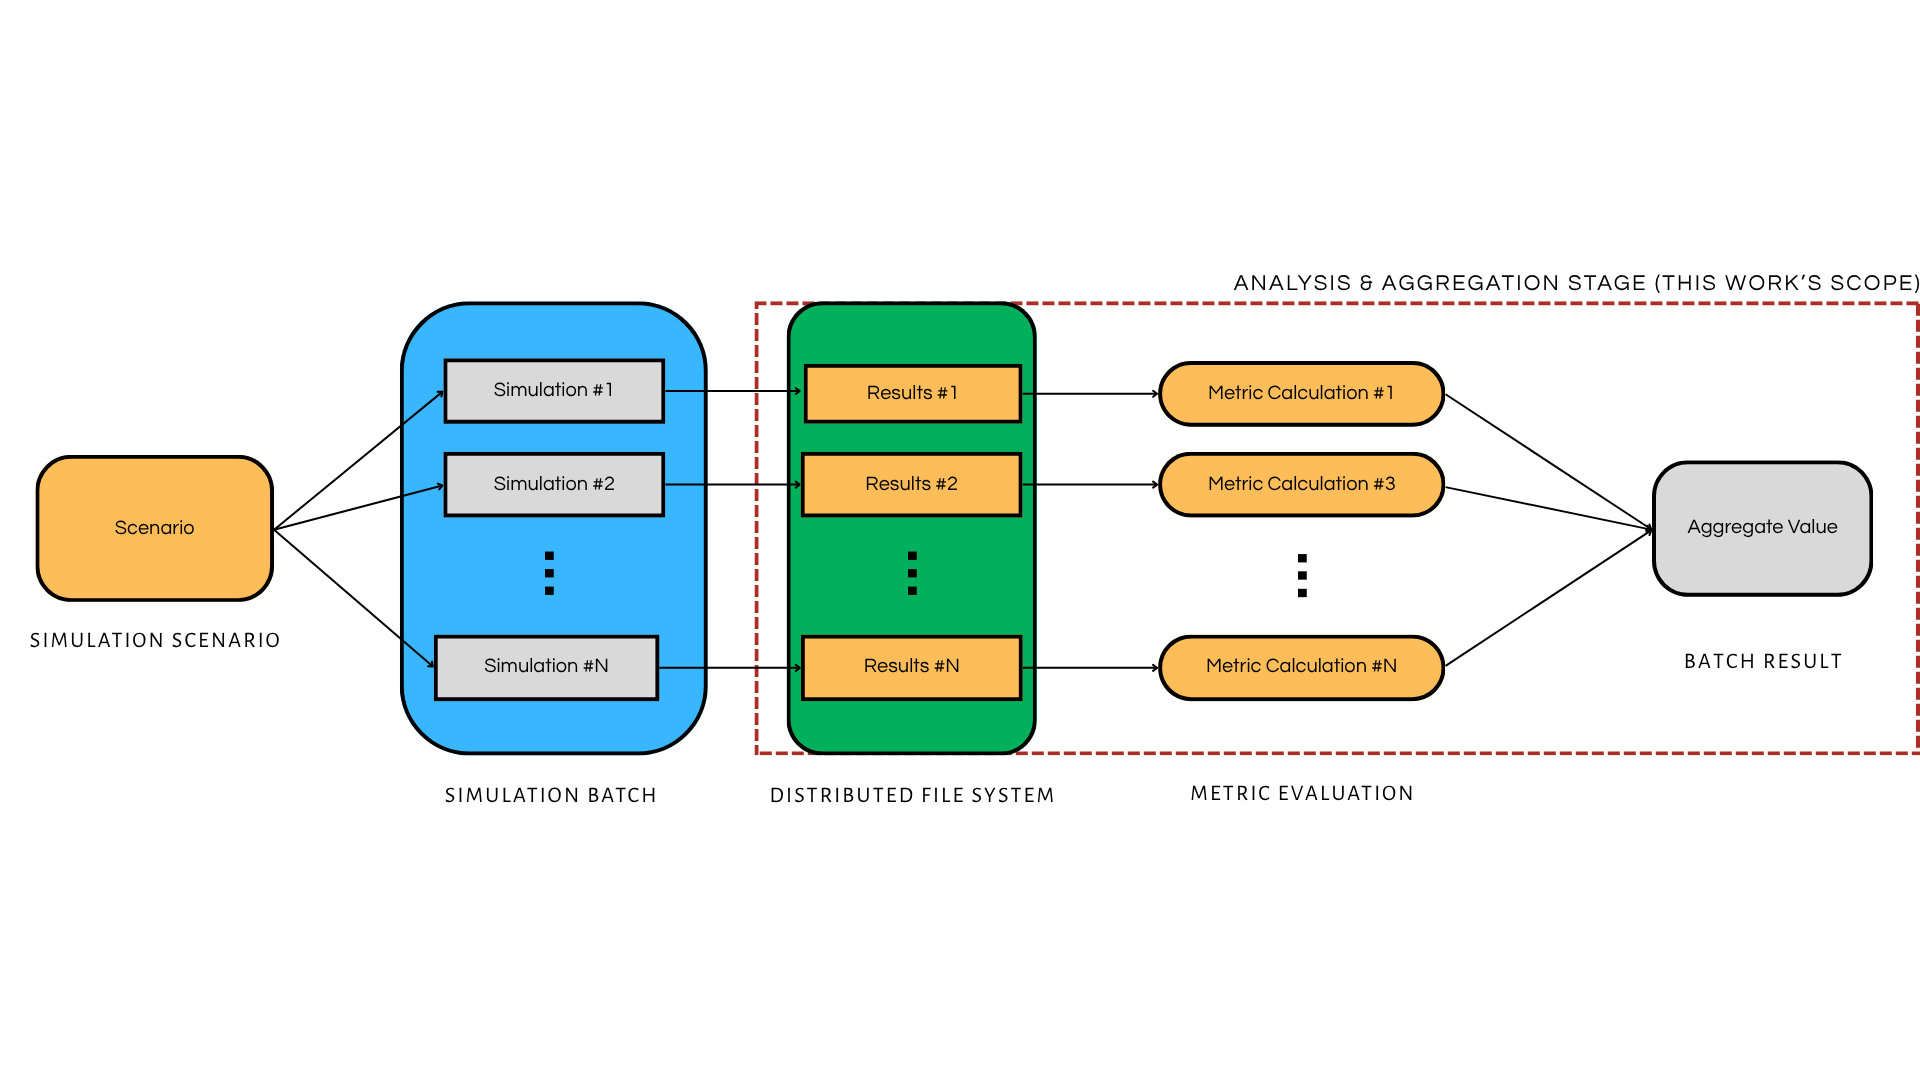
\includegraphics[width=0.82\textwidth]{Cap3/proposed-pipeline.png}
    \caption{Proposed Pipeline.}
    \label{fig:proposed-pipeline}
\end{figure}

This change is expected to improve the pipeline in three ways. First, it reduces unnecessary data movement through the network. Second, it allows independent simulation outputs to be processed concurrently. Third, it makes the analysis stage more consistent with the decision-support role of the overall system, since the user can request analytical products rather than manually orchestrate the intermediate steps. Similar motivations appear in prior work on distributed post-processing and large-scale simulation-data analytics \parencite{li2018postprocessing,morrissey2020velassco,lagares2022aquila}.

The distributed file system is the storage foundation of the proposed architecture. Its role is to persist simulation outputs in a way that supports parallel access and data-local processing. Rather than treating the simulation batch as a monolithic artifact that must be retrieved in full before any computation occurs, the \gls{dfs} allows the output space to be partitioned and accessed by multiple workers. This follows the general principle established in large-scale storage systems such as the Google File System, where reliability, partitioning, and locality are built into the storage design \parencite{ghemawat2003gfs}.

In the context of this thesis, the \gls{dfs} is not introduced as an abstract infrastructure preference, but as a direct response to the analysis bottleneck. If simulation results remain concentrated behind a single retrieval path, post-processing scales poorly. If, instead, the outputs are distributed and directly addressable across the storage layer, the analysis logic can operate on partitions closer to the data source. This makes the \gls{dfs} a necessary enabler of the distributed-processing stage rather than an isolated design choice.

The analytical model proposed in this thesis is based on two stages of transformation. The first stage converts raw outputs from each simulation into metrics. These metrics are run-specific quantities such as survival time, number of losses, or detection-related indicators. The second stage combines those metrics into an aggregate result over the whole batch. Depending on the analytical question, the aggregate result may take the form of an average, a distribution, a ranking, a correlation, or another summary object that supports decision-making.

This distinction is especially important because it gives the analyst explicit control over the semantics of the post-processing workflow. Instead of hard-coding a single output interpretation, the proposed architecture should allow the user to define or select the metric function and the aggregate function before processing begins. This design decision is consistent with the role of sensitivity analysis and scenario comparison in decision support: the same raw outputs may be interpreted differently depending on the question being asked \parencite{wieckowski2023sensitivity}.

The computational strategy behind the proposal can be understood first through the MapReduce lens. At a conceptual level, the map stage corresponds to per-simulation metric extraction, while the reduce stage corresponds to the aggregation of those metrics into a batch-level result \parencite{dean2004mapreduce}. This decomposition is attractive because it mirrors the natural structure of the problem: independent runs first, cross-batch synthesis later.

However, the present thesis also recognizes that the final implementation may benefit from a more flexible \gls{dag}-based engine. Spark, and especially PySpark, provides such a model by representing transformations through lineage and directed acyclic graphs, allowing the analytical plan to be executed as a distributed workflow over partitioned data \parencite{zaharia2012rdd,armbrust2015sparksql}. Therefore, MapReduce serves in this work as a conceptual model for the analytical decomposition, while PySpark is treated as a promising implementation path because it combines distributed execution, structured data handling, and a Python-oriented workflow.

\section{Next Steps}

The first set of next steps concerns research and architectural validation. The selected distributed-processing paradigm must be examined in light of the actual needs of the analysis and aggregation stage. Likewise, the candidate distributed file system must be evaluated not only as a storage technology, but as part of a workflow in which data locality and batch-level post-processing are central concerns. Another research task is to identify metric functions beyond survival time so that the proposed architecture is not tied to a single analytical use case. Finally, the existing \gls{asa} codebase and workflow must be studied in more detail so that integration points can be identified accurately.

The implementation stage follows naturally from those research tasks. A first objective is to create an interface through which the user can define or select an aggregate function together with the simulation batch to be processed. A second objective is to implement a distributed storage layer for the simulation outputs. A third objective is to build the distributed-processing logic that turns persisted results into metrics and aggregate results. After that, the architecture should be tested in a local computer cluster and, if validated, progressively integrated into \gls{asa} systems.

The proposed architecture should be evaluated against the current serial pipeline. At minimum, the evaluation should compare end-to-end processing time for representative simulation batches, identifying how much of the observed gain comes from parallel metric extraction, reduced data transfer, or changes in storage access. It is also important to include qualitative criteria, such as ease of use from the analyst's perspective, the complexity of deployment, and the degree of coupling required between the post-processing layer and the existing \gls{asa} environment.

Because the first implementation will likely be tested in a local cluster, the evaluation must also acknowledge limitations. A local cluster is sufficient to validate the architecture and its workflow logic, but it does not reproduce all the behaviors of a production-grade institutional environment. Therefore, the initial results should be interpreted as architectural validation and preliminary performance evidence rather than as definitive operational benchmarks.

The expected contribution of the complete TG is a software architecture that improves the analysis and aggregation stage of scenario-based simulation outputs by combining distributed storage, distributed processing, and analyst-defined metric semantics. If successful, the resulting system should reduce the need for manual result transfer, shorten the time required to obtain analytical products from simulation batches, and provide a more scalable basis for future work in decision-support workflows built on \gls{asa}.

At a broader level, the thesis also aims to contribute a structured argument for why this problem deserves to be treated independently from simulation execution itself. By framing simulation-output analytics as a first-class architectural problem, the work helps connect decision-support needs in air-defense simulation with contemporary ideas from distributed data processing, scientific workflows, and scalable post-processing systems.
